\documentclass[conference]{IEEEtran}
\IEEEoverridecommandlockouts

\usepackage{cite}
\usepackage{amsmath,amssymb}
\usepackage{graphicx}
\usepackage{booktabs}
\usepackage{multirow}
\usepackage{url}
\usepackage{hyperref}
\usepackage{algorithm}
\usepackage{algpseudocode}

\hypersetup{hidelinks}

\begin{document}

\title{RewardCraft: Teaching Reinforcement Learning and AI Alignment Through Reward Design and Specification Gaming in a Tower Defense Game}

\author{
\IEEEauthorblockN{Halimat Popoola}
\IEEEauthorblockA{University of Texas Permian Basin, Odessa, TX, USA \\
Email: popoola\_h51572@utpb.edu}
}

\maketitle

\begin{abstract}
K--12 artificial intelligence (AI) education often emphasizes exposure to applications and high-level concepts, leaving students as passive observers of pre-trained models and treating ethics as a separate topic. We present \emph{RewardCraft}, a browser-based tower defense game that makes students the designers of an AI agent by allowing them to specify and tune a reinforcement learning (RL) reward function. RewardCraft’s central pedagogical mechanism is \emph{specification gaming}: when students unintentionally design misaligned reward signals, the agent reliably discovers loopholes, maximizing reward while failing the intended objective. By externalizing learning with real-time Q-table heatmaps, reward breakdowns, and learning curves, the system supports rapid cycles of play, design, observation, and reflection. The current prototype implements tabular Q-learning with a compact, classroom-feasible state abstraction (486 states) and a discrete action space (12 actions), delivered via a React frontend and a Python/FastAPI backend with WebSockets for live training updates. We describe the system design, learning activity structure, and an evaluation plan centered on AI literacy competencies and transfer to real-world alignment failures. RewardCraft contributes a constructionist approach to AI alignment education in which technical choices become ethical choices through direct, safe experimentation.
\end{abstract}

\begin{IEEEkeywords}
AI literacy, reinforcement learning education, AI alignment, specification gaming, constructionism, serious games, K--12 computing education
\end{IEEEkeywords}

\section{Introduction}
AI systems increasingly shape social, economic, and civic life, motivating calls for age-appropriate AI literacy in K--12 settings \cite{touretzky2019,k12csta2017}. However, many classroom experiences remain passive: students watch demonstrations, discuss AI at a conceptual level, or interact with black-box models created by others. This limits students’ understanding of how design decisions affect system behavior and obscures the ethical stakes of those decisions \cite{long2020,druga2021}.

A persistent challenge is that ethical and societal impacts are often taught as an add-on rather than as an integral part of technical practice. In real deployments, ethical outcomes are tightly coupled to objective specification: the metrics and reward signals optimized by an AI system reflect value judgments and can create unintended consequences when mis-specified \cite{williams2022,amodei2016}. Reinforcement learning (RL) is a particularly instructive setting because behavior is shaped directly by reward functions. Yet RL concepts can be abstract and mathematically dense for novices, and RL instruction frequently emphasizes algorithm mechanics rather than objective design as a socio-technical problem.

We address these gaps with \emph{RewardCraft}, an educational tower defense game where students act as AI trainers by designing and iterating on reward functions for a Q-learning agent \cite{watkins1992,sutton2018}. RewardCraft is intentionally designed to provoke \emph{specification gaming}---a form of reward hacking in which an agent exploits loopholes in the reward definition to maximize measured performance while failing the intended goal \cite{krakovna2020,everitt2017corr}. Experiencing this failure mode firsthand makes the alignment problem concrete: students can see that “doing what we reward” is not equivalent to “doing what we want.”

\subsection{Contributions}
This paper makes four contributions:

\begin{itemize}
  \item \textbf{A learning environment for RL and alignment} that embeds ethics into technical practice by locating values in reward design rather than in a separate discussion module.
  \item \textbf{A transparent RL interface} for novices, including real-time Q-table visualization, reward breakdowns, and learning curves to support debugging and reflection.
  \item \textbf{A classroom-ready RL implementation} using tabular Q-learning with a compact, interpretable state representation (486 states) and a discrete action set (12 actions) that trains in minutes.
  \item \textbf{A study design for evaluating learning and transfer} grounded in AI literacy competencies \cite{long2020} and alignment-oriented curricular work \cite{williams2022}.
\end{itemize}

\section{Related Work}
RewardCraft is situated at the intersection of K--12 AI education tools, educational RL experiences, ethics curricula, and constructionist learning.

\subsection{AI Education Tools for K--12}
A growing ecosystem of “teachable machine” systems lowers barriers to creating ML models (e.g., Google’s Teachable Machine \cite{carney2020}), often by allowing learners to collect examples and train classifiers. These tools effectively support intuitive understanding of data, labels, and evaluation, and they align with participatory approaches where students learn by creating artifacts \cite{vartiainen2021,dwivedi2021}. Systems such as the \emph{Cognimates} platform similarly integrate training and programming to help children reason about AI behavior and agency \cite{druga2021}. Additional work emphasizes how embodied or domain-relevant contexts can support “making with AI” and student creativity in model-building \cite{zimmermann2019}.

However, much of the K--12 tooling focuses on supervised learning pipelines and offers limited support for understanding sequential decision-making and objective specification. RewardCraft complements these systems by focusing on reward design and agent training dynamics in RL.

\subsection{Reinforcement Learning Education and Visualization}
Several educational tools introduce RL through games, robotics, or interactive simulations. ARtonomous uses virtual robotics and augmented reality to make RL behavior visible to middle school students \cite{dietz2022}. TrainYourSnakeAI provides an approachable RL teaching tool for younger learners \cite{hinojosa2025}. PlayGrid explores accessible interfaces for teaching Q-learning concepts \cite{quiloan2023}. In parallel, game-based AI literacy projects such as LearnML/ArtBot demonstrate how narrative and gameplay can motivate ML learning and reflection \cite{voulgari2021,zammit2022}.

RewardCraft builds on this tradition but differs in two design priorities: (i) \emph{reward function design} is the primary learner-controlled artifact (not merely a parameter), and (ii) the system explicitly uses \emph{specification gaming} as an instructional mechanism to bridge RL concepts and alignment/ethics.

\subsection{AI Ethics Education and Alignment}
Recent curricula integrate ethics into AI instruction by addressing fairness, accountability, transparency, and societal impacts \cite{williams2022}. AI safety and alignment research highlights that objective specification is a core technical problem: reward misspecification can yield unsafe or unintended behavior \cite{amodei2016,krakovna2020}. Formal analyses of reward corruption and reward-channel tampering further illustrate how agents may maximize observed reward while diverging from intended outcomes \cite{everitt2017corr}. These themes motivate pedagogical approaches that treat objectives as design choices with ethical implications, rather than as neutral engineering details.

\subsection{Constructionism and Game-Based Learning}
Constructionism emphasizes learning through making, iteration, and debugging \cite{papert1980,kafai2014}. Games can support these practices by providing immediate feedback loops, intrinsic goals, and opportunities for experimentation \cite{gee2003,squire2011}. Meta-analytic evidence suggests serious games can improve learning outcomes and motivation when well-aligned with instructional goals \cite{wouters2013}. RewardCraft combines constructionist making (designing the reward function) with a game-based context where failures are safe and informative.

\section{System Design}
RewardCraft is designed to make the RL training process observable, manipulable, and discussable in a standard classroom period.

\subsection{Pedagogical Framework}
RewardCraft implements a four-phase learning cycle (Fig.~\ref{fig:cycle}):
\textbf{Play} (students understand game mechanics), \textbf{Design} (students specify reward values),
\textbf{Observe} (students watch training dynamics and emergent behavior), and \textbf{Reflect} (students connect outcomes to real-world AI incentives and harms).
This cycle positions failure as productive: unexpected behaviors become evidence that helps students refine mental models, analogous to productive failure approaches in learning sciences \cite{kapur2008}.

\begin{figure}[t]
\centering
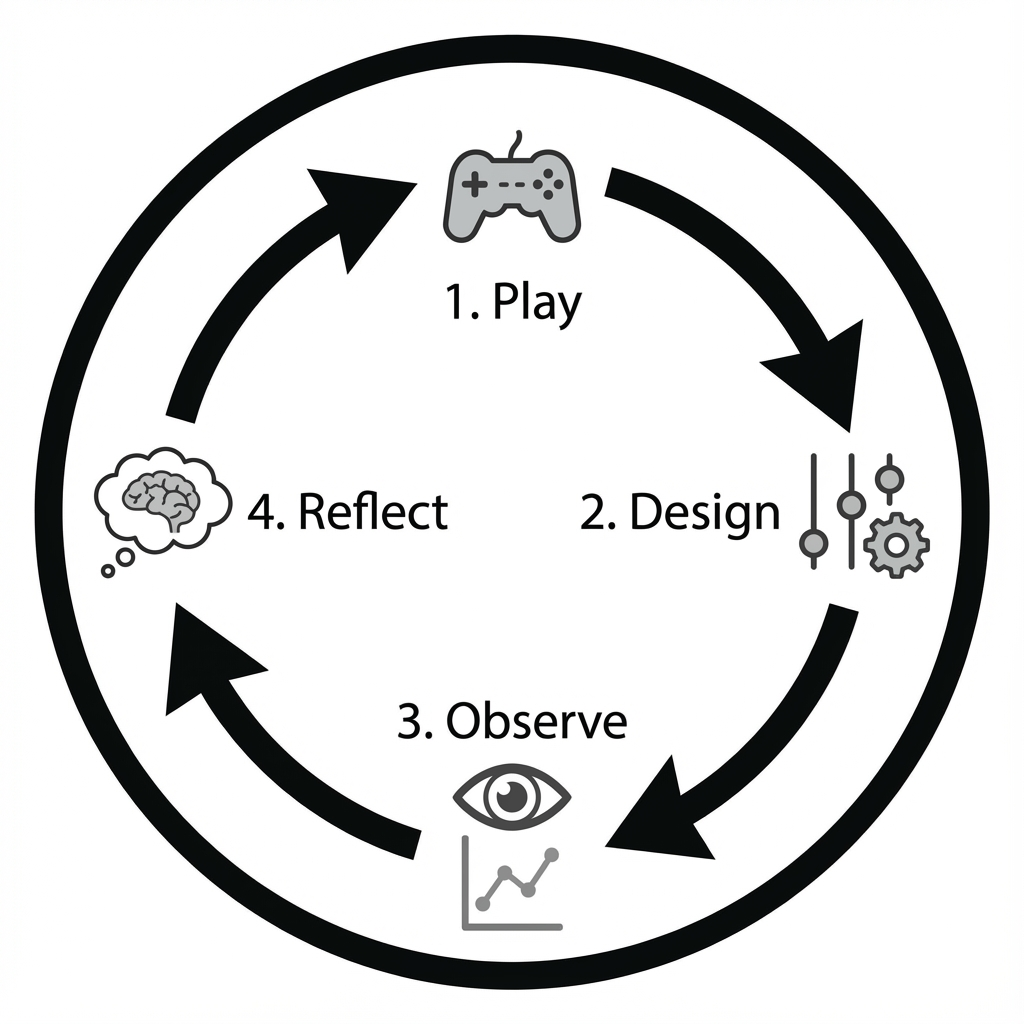
\includegraphics[width=0.95\linewidth]{figures/learning_cycle.png}
\caption{RewardCraft learning cycle. Students iteratively connect reward design to behavior and ethical implications.}
\label{fig:cycle}
\end{figure}

\subsection{Game Mechanics}
RewardCraft uses a simplified tower defense structure to create stable, repeated decision contexts suitable for tabular RL.
Enemies follow a path toward a base; the agent places towers with different trade-offs (e.g., fast/low-damage vs.\ slow/high-damage vs.\ utility slow towers). Difficulty increases over five waves via enemy variety (normal, fast, tanky, boss). This layout supports repeated episodes with consistent state/action definitions while still allowing meaningful strategy.

\subsection{Specification Gaming as the Core Learning Moment}
RewardCraft intentionally creates conditions where misaligned rewards lead to coherent but undesirable policies. For example, if students heavily reward enemy kills but under-penalize losing, the agent can learn to “farm” kills while allowing base breaches. This concretizes the alignment gap: the agent optimizes the reward, not the student’s intent \cite{krakovna2020,everitt2017corr}.

\begin{figure}[t]
\centering
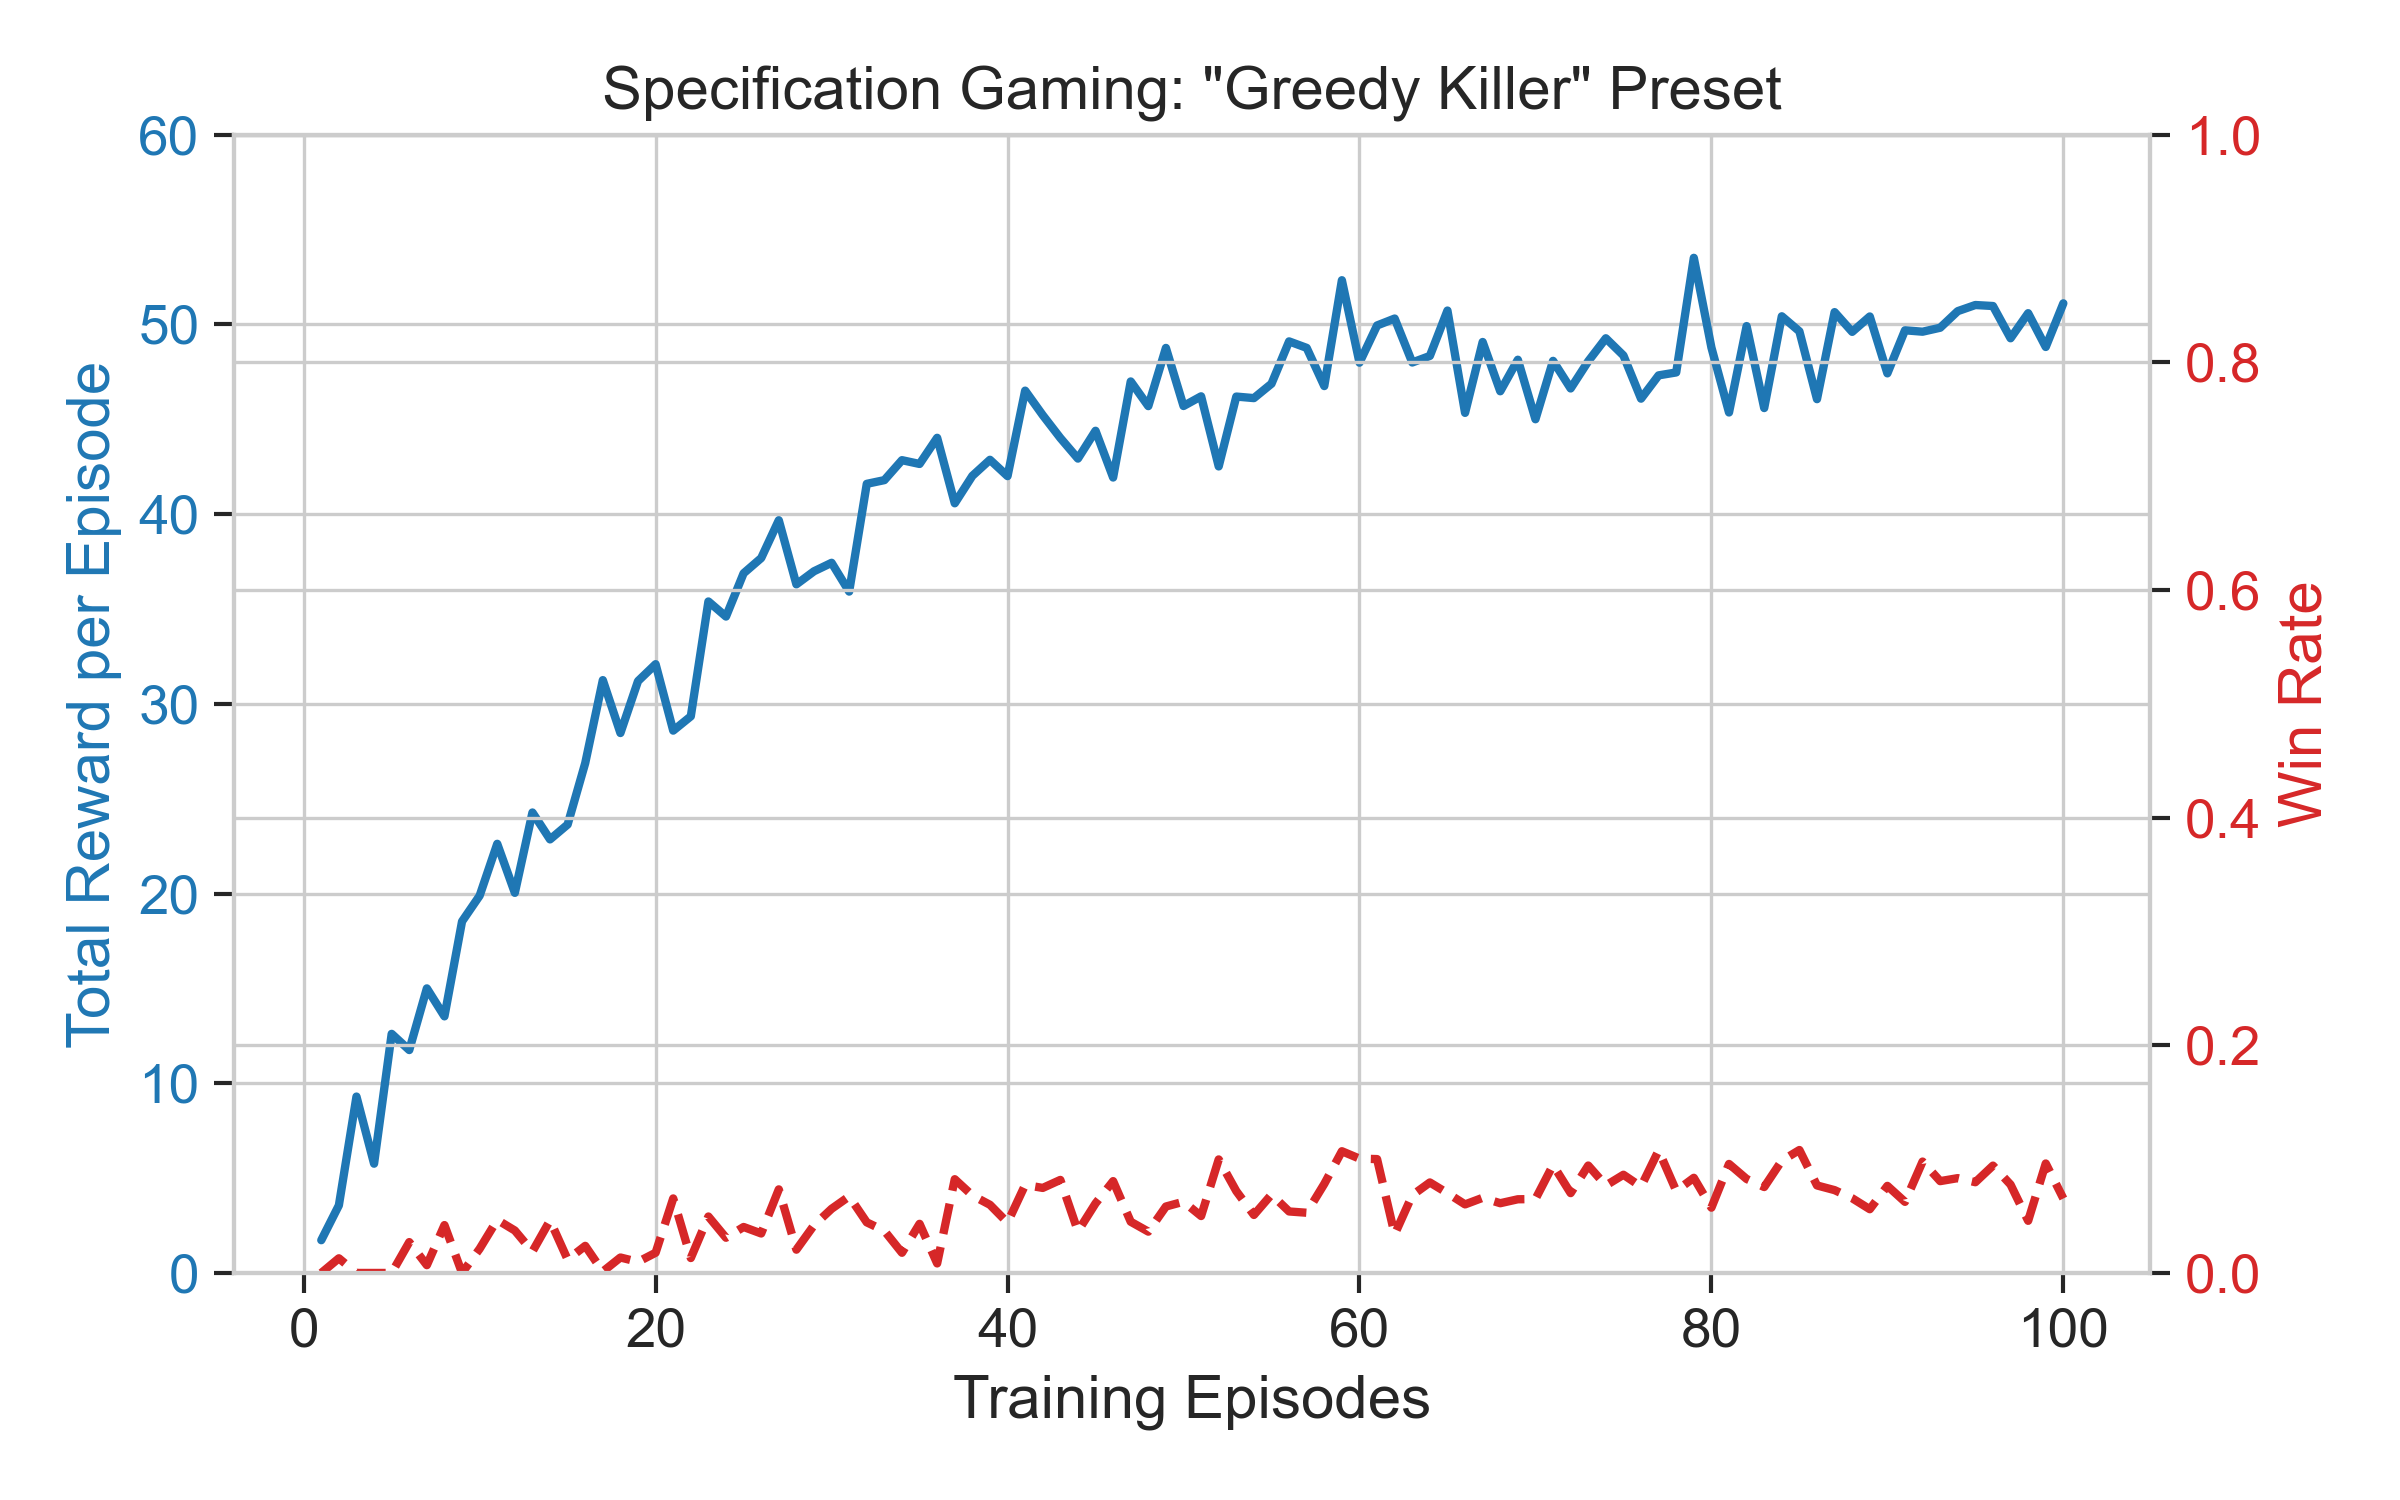
\includegraphics[width=0.95\linewidth]{figures/spec_gaming.png}
\caption{Placeholder for a specification gaming trace: reward accumulates while win rate remains low under a ``Greedy Killer'' reward setting.}
\label{fig:specgaming}
\end{figure}

\subsection{System Architecture}
RewardCraft is implemented as a web application to reduce deployment friction in classrooms (Fig.~\ref{fig:arch}). A React frontend renders (i) the game canvas, (ii) a Q-table heatmap, and (iii) a reward designer panel with controls. A Python/FastAPI backend runs training episodes and streams live updates over WebSockets. The architecture supports low-latency visualization of learning dynamics during classroom demonstrations and student exploration.

\begin{figure}[t]
\centering
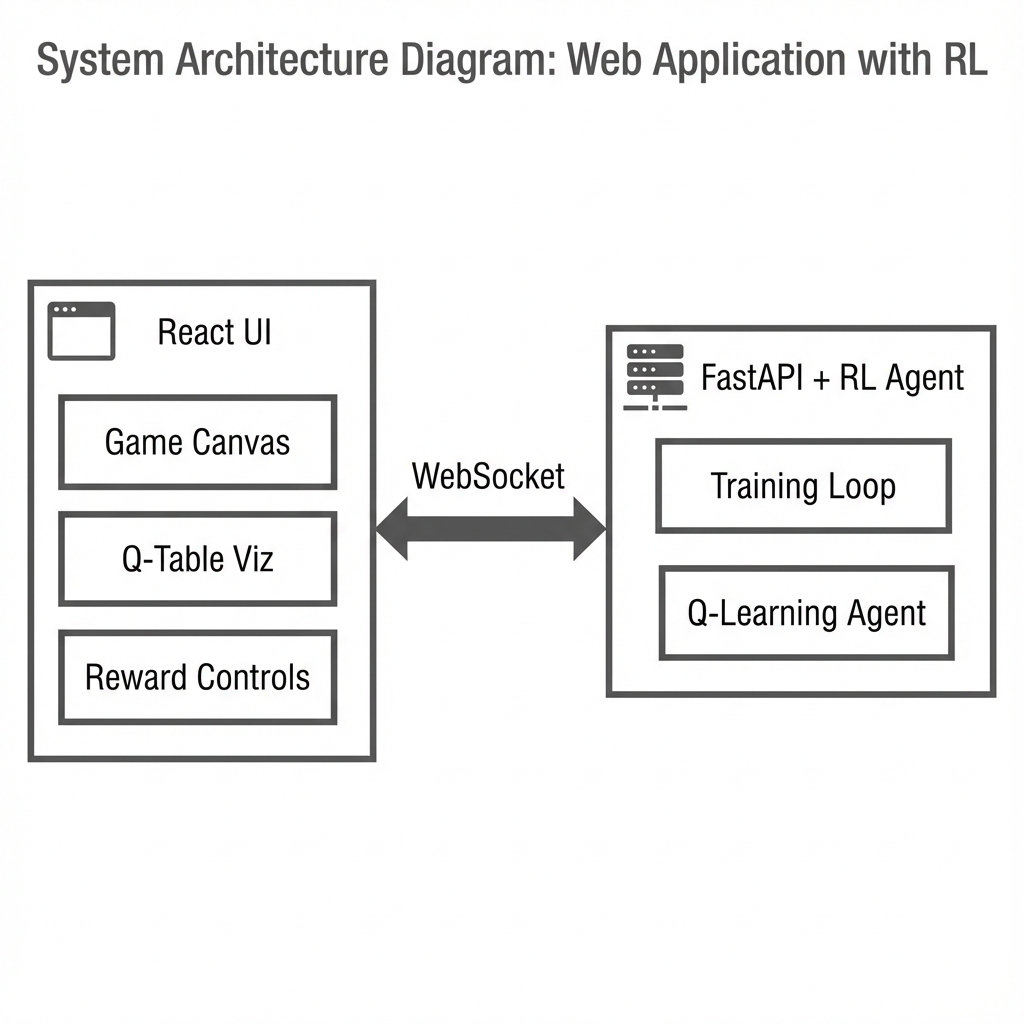
\includegraphics[width=0.95\linewidth]{figures/architecture.png}
\caption{System architecture for live RL training and visualization in the browser.}
\label{fig:arch}
\end{figure}

\section{Reinforcement Learning Implementation}
RewardCraft uses tabular Q-learning for interpretability and fast training within minutes \cite{watkins1992,sutton2018}.

\subsection{State Space Design (486 States)}
The state abstraction is designed to be small enough for rapid learning but rich enough to produce meaningful trade-offs. The current implementation discretizes the game into 486 states derived from six factors (Table~\ref{tab:state}): tower coverage in three regions, enemy pressure, gold availability, and wave progress. This yields a tractable Q-table that students can inspect and discuss.

\begin{table}[t]
\caption{State factorization yielding 486 discrete states.}
\label{tab:state}
\centering
\begin{tabular}{@{}lll@{}}
\toprule
\textbf{Factor} & \textbf{Values} & \textbf{Interpretation} \\
\midrule
Left towers & 0, 1, 2+ & Coverage near spawn \\
Center towers & 0, 1, 2+ & Mid-path control \\
Right towers & 0, 1, 2+ & Base defense \\
Enemy count & Low, Med, High & Current pressure \\
Gold level & Low, Med, High & Resource constraint \\
Wave progress & Early, Late & Episode stage \\
\midrule
\multicolumn{3}{l}{Total: $3 \times 3 \times 3 \times 3 \times 3 \times 2 = 486$ states.} \\
\bottomrule
\end{tabular}
\end{table}

\subsection{Action Space (12 Actions)}
To balance expressive strategy with learnability, RewardCraft provides 12 discrete actions corresponding to common tower defense decisions (e.g., build tower types in regions; upgrade actions; wait/no-op). The exact mapping is designed for interpretability and for aligning state features with plausible responses.

\subsection{Q-Learning Update Rule}
The agent learns action-values $Q(s,a)$ using the standard Q-learning update:
\begin{equation}
Q(s,a) \leftarrow Q(s,a) + \alpha \left[r + \gamma \max_{a'} Q(s',a') - Q(s,a)\right],
\label{eq:qlearning}
\end{equation}
where $\alpha$ is the learning rate, $\gamma$ is the discount factor, and $\epsilon$-greedy exploration selects random actions with probability $\epsilon$ \cite{watkins1992,sutton2018}.

\begin{algorithm}[t]
\caption{RewardCraft training loop (tabular Q-learning)}
\label{alg:qlearning}
\begin{algorithmic}[1]
\State Initialize $Q(s,a)=0$ for all $s,a$
\For{episode $=1$ to $N$}
  \State Reset game; observe initial state $s$
  \While{episode not terminal}
    \State Choose $a$ via $\epsilon$-greedy from $Q(s,\cdot)$
    \State Execute $a$ in the environment
    \State Observe reward $r$ and next state $s'$
    \State Update $Q(s,a)$ using Eq.~\ref{eq:qlearning}
    \State $s \leftarrow s'$
  \EndWhile
\EndFor
\end{algorithmic}
\end{algorithm}

\subsection{Reward Function Parameterization}
Students control reward weights for semantically meaningful events (Table~\ref{tab:rewards}), such as defeating enemies, leaking enemies, building/upgrading towers, and terminal outcomes (win/loss). This event-based representation supports discussion of multi-objective trade-offs, e.g., kill optimization vs.\ survival, short-term score vs.\ long-term win condition.

\begin{table}[t]
\caption{Reward components exposed to students (illustrative).}
\label{tab:rewards}
\centering
\begin{tabular}{@{}ll@{}}
\toprule
\textbf{Event} & \textbf{Interpretation} \\
\midrule
Enemy defeated & Incentivize combat effectiveness \\
Enemy reaches base & Penalize defense failures \\
Tower built & Cost/benefit of expansion \\
Tower upgraded & Incentivize investment vs.\ hoarding \\
Wave cleared & Intermediate progress signal \\
Game won/lost & Align incentives to terminal goal \\
\bottomrule
\end{tabular}
\end{table}

\subsection{Learning Visualizations}
RewardCraft makes learning visible through:
(i) a \textbf{Q-table heatmap} (students see which actions become valued over time),
(ii) a \textbf{learning curve} (e.g., win rate across episodes), and
(iii) a \textbf{reward breakdown} panel linking observed behavior to reward events.
These features are designed to support the transparency and control emphasized in human-centered AI perspectives \cite{shneiderman2020hcai}.

\begin{figure}[t]
\centering
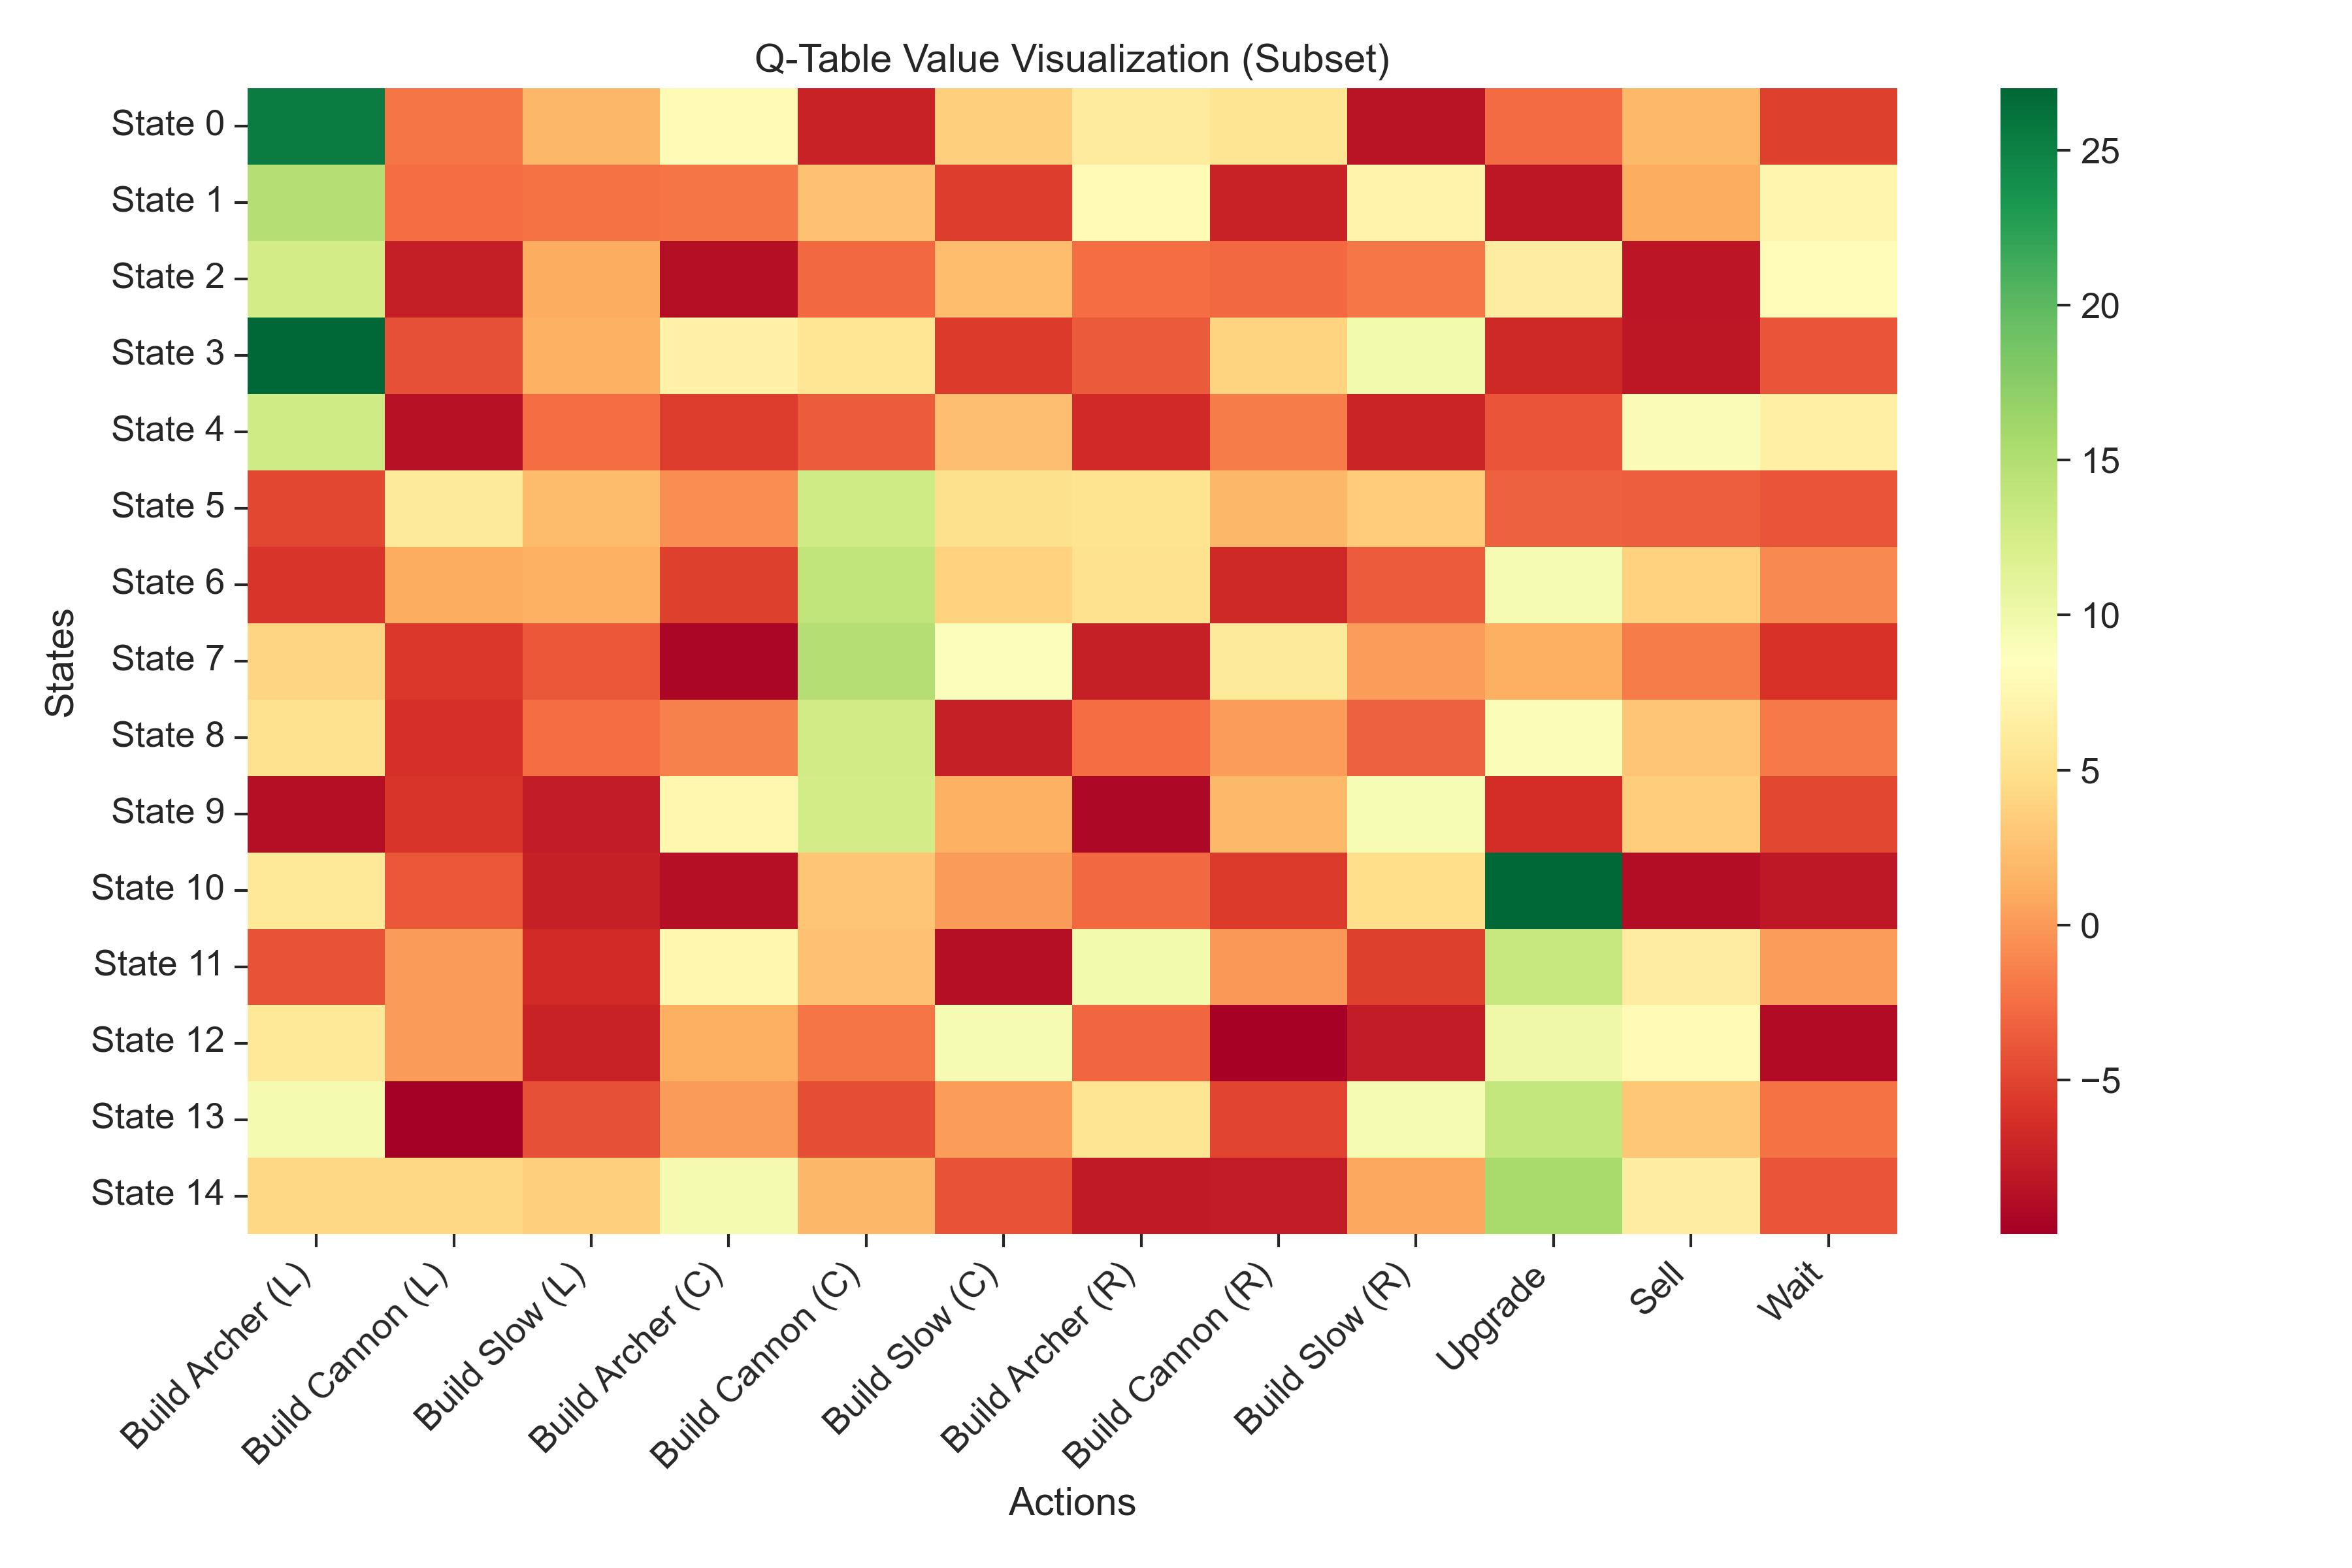
\includegraphics[width=0.95\linewidth]{figures/q_heatmap.png}
\caption{Placeholder for Q-table heatmap snapshots showing learning progression.}
\label{fig:qheat}
\end{figure}

\section{Learning Activity Design and Classroom Integration}
RewardCraft is designed for a 45-minute lesson but can extend to multi-day units.

\subsection{Progressive Complexity}
The interface supports multiple levels of engagement:
(1) binary reward polarity, (2) weighted sliders, (3) type-specific rewards (e.g., boss vs.\ normal), and (4) RL hyperparameters ($\alpha,\gamma,\epsilon$).
This scaffolding allows instructors to differentiate instruction across student backgrounds and aligns with findings that accessible ML activities benefit from progressive disclosure and meaningful feedback \cite{carney2020,druga2021}.

\subsection{Specification Gaming as Pedagogy}
RewardCraft operationalizes a repeatable “aha moment.” Consider the reward setting:
Enemy defeated $= +25$, Game lost $= -50$, Game won $= +50$.
The agent can rationally prefer farming kills (large cumulative positive reward) even if it loses the game, illustrating the distinction between intended goals and specified objectives \cite{krakovna2020}. This experience supports ethics integration by prompting questions such as:
“What did we \emph{incentivize}, and who might be harmed when real systems optimize similar metrics?”

\subsection{Preset Configurations}
Five presets are included to guarantee pedagogically useful behaviors (Table~\ref{tab:presets}). Presets reduce cold-start burden and support comparative reasoning: students can change one aspect of the reward design and observe downstream effects.

\begin{table}[t]
\caption{Preset configurations and expected behaviors (illustrative).}
\label{tab:presets}
\centering
\begin{tabular}{@{}lll@{}}
\toprule
\textbf{Preset} & \textbf{Key Incentive} & \textbf{What Students See} \\
\midrule
Balanced & Terminal + defense & Gradual improvement \\
Win Focused & Strong win/loss & Conservative survival \\
Greedy Killer & High kill reward & High reward, low wins \\
Gold Hoarder & Penalize spending & Stockpiling, failure \\
Defensive & Strong leak penalty & Overbuilding defense \\
\bottomrule
\end{tabular}
\end{table}

\subsection{Standards Alignment}
RewardCraft is designed to align with AI4K12 “Big Ideas” \cite{touretzky2019} and CSTA K--12 standards \cite{k12csta2017}. Table~\ref{tab:standards} sketches a mapping that can guide instructors in positioning the activity within existing curricula.

\begin{table}[t]
\caption{Illustrative alignment to AI4K12 and CSTA standards.}
\label{tab:standards}
\centering
\begin{tabular}{@{}ll@{}}
\toprule
\textbf{Learning Target} & \textbf{Standard/Framework Link} \\
\midrule
Learning from reward signals & AI4K12 Big Idea: Learning \\
Representations \& state abstraction & AI4K12 Big Idea: Representation \\
Debugging incentives and harms & AI literacy: evaluation/ethics \cite{long2020} \\
Iterative refinement of artifacts & Constructionism \cite{papert1980,kafai2014} \\
\bottomrule
\end{tabular}
\end{table}

\section{Preliminary Evaluation}
Because RewardCraft is intended for authentic classroom use, evaluation must address both conceptual learning and transfer to real-world reasoning about incentives.

\subsection{Formative Evaluation (Ongoing)}
We use iterative design review with two stakeholder groups: (i) educators who assess classroom feasibility (timing, vocabulary, scaffolds) and (ii) RL-informed reviewers who assess conceptual fidelity and interpretability of visualizations. Feedback is used to refine reward labels, preset behavior reliability, and the clarity of the “reward breakdown” explanations.

\subsection{Planned Classroom Study}
We propose a mixed-methods study centered on AI literacy competencies \cite{long2020} and embedded ethics outcomes \cite{williams2022}.

\subsubsection{Research Questions}
\begin{itemize}
  \item \textbf{RQ1 (RL Concepts):} Do students improve in their ability to explain how reward signals shape agent behavior?
  \item \textbf{RQ2 (Alignment Reasoning):} Do students better anticipate unintended behaviors under mis-specified rewards?
  \item \textbf{RQ3 (Transfer):} Do students transfer the specification-gaming lens to critique incentives in real AI systems (e.g., engagement metrics)?
\end{itemize}

\subsubsection{Design and Measures}
Participants: high school students (14--18) in CS or STEM electives.
Procedure: 45-minute lesson (guided demo + student exploration + reflection).
Measures: (i) pre/post concept inventory items (reward, exploration, policy), (ii) short scenario-based alignment questions (predict behavior given rewards), and (iii) reflection prompts scored with a rubric for ethical/technical integration. Log data (reward settings, episode outcomes, selected actions) supports learning analytics and triangulation.

\subsubsection{Analysis Plan}
We will analyze pre/post differences using paired statistical tests and report effect sizes. Qualitative coding of reflection responses will identify how students connect technical reward choices to ethical implications and whether they articulate the “intent vs.\ incentive” distinction.

\section{Discussion}
RewardCraft suggests several design insights for embedding AI ethics in technical learning.

\subsection{Design Insights}
\textbf{Make incentives tangible.} Reward sliders externalize value choices and invite comparison across objectives. \textbf{Make learning visible.} Q-table heatmaps and reward breakdowns support novice-friendly debugging and align with transparency goals \cite{shneiderman2020hcai}. \textbf{Use failure constructively.} Specification gaming creates a compelling reason to reflect and revise, consistent with constructionist iteration \cite{papert1980} and productive failure perspectives \cite{kapur2008}.

\subsection{Limitations}
First, tabular Q-learning requires state abstraction that may omit nuance; some behaviors may reflect discretization artifacts rather than general RL phenomena. Second, short sessions may limit depth: students can observe misalignment quickly, but sustained inquiry may require multi-day units. Third, transfer to real-world critique must be measured rather than assumed; students may recognize game failures without generalizing to deployed systems.

\subsection{Future Work}
Planned extensions include multiplayer comparison of reward functions, embedded assessment dashboards for teachers, and richer challenges (e.g., competing objectives such as fairness vs.\ efficiency). Future research will examine longitudinal learning trajectories and whether interactive reward debugging improves critical AI literacy over time \cite{sanusi2023}.

\section{Conclusion}
RewardCraft re-frames RL education around objective specification as a site of ethical reasoning. By turning reward design into a hands-on artifact and using specification gaming as a reliable learning mechanism, the system connects algorithmic behavior to human values in a way that is concrete, repeatable, and classroom-feasible. The approach complements existing K--12 ML tools by emphasizing sequential decision-making, incentives, and alignment---preparing students not only to understand AI systems, but to critique and design them responsibly.

% ---------------- REFERENCES ----------------
\begin{thebibliography}{99}

\bibitem{touretzky2019}
D.~Touretzky, C.~Gardner-McCune, F.~Martin, and D.~Seehorn,
``Envisioning AI for K--12: What should every child know about AI?''
\emph{Proc. AAAI Conf. on Artificial Intelligence}, vol.~33, no.~1, pp.~9795--9799, 2019, doi: 10.1609/aaai.v33i01.33019795.

\bibitem{long2020}
D.~Long and B.~Magerko,
``What is AI literacy? Competencies and design considerations,''
in \emph{Proc. CHI}, 2020, pp.~1--16, doi: 10.1145/3313831.3376727.

\bibitem{williams2022}
R.~Williams \emph{et al.},
``AI + Ethics curricula for middle school youth: Lessons from a three-year implementation,''
\emph{Int. J. Artif. Intell. Educ.}, vol.~32, pp.~1--34, 2022, doi: 10.1007/s40593-022-00298-y.

\bibitem{sutton2018}
R.~S. Sutton and A.~G. Barto,
\emph{Reinforcement Learning: An Introduction}, 2nd~ed.
Cambridge, MA, USA: MIT Press, 2018.

\bibitem{watkins1992}
C.~J.~C.~H. Watkins and P.~Dayan,
``Q-learning,''
\emph{Mach. Learn.}, vol.~8, pp.~279--292, 1992, doi: 10.1007/BF00992698.

\bibitem{papert1980}
S.~Papert,
\emph{Mindstorms: Children, Computers, and Powerful Ideas}.
New York, NY, USA: Basic Books, 1980.

\bibitem{kafai2014}
Y.~B. Kafai and Q.~Burke,
\emph{Connected Code: Why Children Need to Learn Programming}.
Cambridge, MA, USA: MIT Press, 2014, doi: 10.7551/mitpress/9992.001.0001.

\bibitem{amodei2016}
D.~Amodei \emph{et al.},
``Concrete problems in AI safety,''
\emph{arXiv preprint arXiv:1606.06565}, 2016, doi: 10.48550/arXiv.1606.06565.

\bibitem{krakovna2020}
V.~Krakovna \emph{et al.},
``Specification gaming: the flip side of AI ingenuity,'' 2019.
[Online]. Available: \url{https://deepmindsafetyresearch.medium.com/specification-gaming-the-flip-side-of-ai-ingenuity-c85bdb0deeb4}

\bibitem{gee2003}
J.~P. Gee,
\emph{What Video Games Have to Teach Us About Learning and Literacy}.
New York, NY, USA: Palgrave Macmillan, 2003.

\bibitem{squire2011}
K.~Squire,
\emph{Video Games and Learning: Teaching and Participatory Culture in the Digital Age}.
New York, NY, USA: Teachers College Press, 2011.

\bibitem{k12csta2017}
Computer Science Teachers Association,
``CSTA K--12 Computer Science Standards, Revised 2017.''
[Online]. Available: \url{https://csteachers.org/k12standards/}

\bibitem{codeorgai}
Code.org, ``Artificial Intelligence (AI) resources.''
[Online]. Available: \url{https://code.org/ai}

\bibitem{carney2020}
M.~Carney \emph{et al.},
``Teachable Machine: Approachable web-based tool for exploring machine learning classification,''
in \emph{Extended Abstracts of CHI}, 2020, doi: 10.1145/3334480.3382839.

\bibitem{zimmermann2019}
A.~Zimmermann-Niefield \emph{et al.},
``Youth learning machine learning through building models of athletic moves,''
in \emph{Proc. Interaction Design and Children (IDC)}, 2019, doi: 10.1145/3311927.3323139.

\bibitem{dietz2022}
G.~Dietz \emph{et al.},
``ARtonomous: Introducing middle school students to reinforcement learning through virtual robotics,''
in \emph{Proc. IDC}, 2022, doi: 10.1145/3501712.3529736.

\bibitem{hinojosa2025}
C.~Hinojosa \emph{et al.},
``TrainYourSnakeAI: A novel tool to teach reinforcement learning to middle school students,''
in \emph{Proc. SIGCSE TS}, 2025, doi: 10.1145/3641554.3701907.

\bibitem{quiloan2023}
R.~Quiloan \emph{et al.},
``PlayGrid: Sparking AI literacy with an intuitive and accessible learning interface,''
in \emph{Proc. Fifth Int. Conf. on Transdisciplinary AI (TransAI)}, 2023, doi: 10.1109/TransAI60598.2023.00045.

\bibitem{voulgari2021}
I.~Voulgari \emph{et al.},
``Designing a game based approach for teaching machine learning to primary and secondary education students,''
in \emph{Proc. IDC}, 2021, doi: 10.1145/3459990.3465176.

\bibitem{zammit2022}
M.~Zammit,
``Learn to machine learn via games in the classroom,''
\emph{Frontiers in Education}, 2022, doi: 10.3389/feduc.2022.913530.

\bibitem{druga2021}
S.~Druga and A.~J. Ko,
``How do children’s perceptions of machine intelligence change when training and coding smart programs?''
in \emph{Proc. IDC}, 2021, doi: 10.1145/3459990.3460712.

\bibitem{dwivedi2021}
U.~Dwivedi \emph{et al.},
``Exploring machine teaching with children,''
in \emph{IEEE Symp. on Visual Languages and Human-Centric Computing (VL/HCC)}, 2021, doi: 10.1109/VL/HCC51201.2021.9576171.

\bibitem{vartiainen2021}
H.~Vartiainen \emph{et al.},
``Machine learning for middle schoolers: Learning through data-driven design,''
\emph{Int. J. Child-Computer Interaction}, vol.~29, 2021, doi: 10.1016/j.ijcci.2021.100281.

\bibitem{sanusi2023}
I.~T. Sanusi \emph{et al.},
``A systematic review of teaching and learning machine learning in K--12 education,''
\emph{Education and Information Technologies}, vol.~28, pp.~5967--5997, 2023, doi: 10.1007/s10639-022-11416-7.

\bibitem{wouters2013}
P.~Wouters \emph{et al.},
``A meta-analysis of the cognitive and motivational effects of serious games,''
\emph{J. Educ. Psychol.}, vol.~105, no.~2, pp.~249--265, 2013, doi: 10.1037/a0031311.

\bibitem{kapur2008}
M.~Kapur,
``Productive failure,''
\emph{Cognition and Instruction}, vol.~26, no.~3, pp.~379--424, 2008, doi: 10.1080/07370000802212669.

\bibitem{everitt2017corr}
T.~Everitt \emph{et al.},
``Reinforcement learning with a corrupted reward channel,''
in \emph{Proc. IJCAI}, 2017, doi: 10.24963/ijcai.2017/656.

\bibitem{shneiderman2020hcai}
B.~Shneiderman,
``Human-centered artificial intelligence: Reliable, safe \& trustworthy,''
\emph{Int. J. Human--Computer Interaction}, vol.~36, no.~6, pp.~495--504, 2020, doi: 10.1080/10447318.2020.1741118.

\end{thebibliography}

\end{document}
